\documentclass[11pt]{scrartcl}\usepackage[]{graphicx}\usepackage[]{color}
%% maxwidth is the original width if it is less than linewidth
%% otherwise use linewidth (to make sure the graphics do not exceed the margin)
\makeatletter
\def\maxwidth{ %
  \ifdim\Gin@nat@width>\linewidth
    \linewidth
  \else
    \Gin@nat@width
  \fi
}
\makeatother

\definecolor{fgcolor}{rgb}{0.345, 0.345, 0.345}
\newcommand{\hlnum}[1]{\textcolor[rgb]{0.686,0.059,0.569}{#1}}%
\newcommand{\hlstr}[1]{\textcolor[rgb]{0.192,0.494,0.8}{#1}}%
\newcommand{\hlcom}[1]{\textcolor[rgb]{0.678,0.584,0.686}{\textit{#1}}}%
\newcommand{\hlopt}[1]{\textcolor[rgb]{0,0,0}{#1}}%
\newcommand{\hlstd}[1]{\textcolor[rgb]{0.345,0.345,0.345}{#1}}%
\newcommand{\hlkwa}[1]{\textcolor[rgb]{0.161,0.373,0.58}{\textbf{#1}}}%
\newcommand{\hlkwb}[1]{\textcolor[rgb]{0.69,0.353,0.396}{#1}}%
\newcommand{\hlkwc}[1]{\textcolor[rgb]{0.333,0.667,0.333}{#1}}%
\newcommand{\hlkwd}[1]{\textcolor[rgb]{0.737,0.353,0.396}{\textbf{#1}}}%
\let\hlipl\hlkwb

\usepackage{framed}
\makeatletter
\newenvironment{kframe}{%
 \def\at@end@of@kframe{}%
 \ifinner\ifhmode%
  \def\at@end@of@kframe{\end{minipage}}%
  \begin{minipage}{\columnwidth}%
 \fi\fi%
 \def\FrameCommand##1{\hskip\@totalleftmargin \hskip-\fboxsep
 \colorbox{shadecolor}{##1}\hskip-\fboxsep
     % There is no \\@totalrightmargin, so:
     \hskip-\linewidth \hskip-\@totalleftmargin \hskip\columnwidth}%
 \MakeFramed {\advance\hsize-\width
   \@totalleftmargin\z@ \linewidth\hsize
   \@setminipage}}%
 {\par\unskip\endMakeFramed%
 \at@end@of@kframe}
\makeatother

\definecolor{shadecolor}{rgb}{.97, .97, .97}
\definecolor{messagecolor}{rgb}{0, 0, 0}
\definecolor{warningcolor}{rgb}{1, 0, 1}
\definecolor{errorcolor}{rgb}{1, 0, 0}
\newenvironment{knitrout}{}{} % an empty environment to be redefined in TeX

\usepackage{alltt}

\setlength{\oddsidemargin}{0in}  %left margin position, reference is one inch
\setlength{\textwidth}{6.5in}    %width of text=8.5-1in-1in for margin
\setlength{\topmargin}{-0.5in}    %reference is at 1.5in, -.5in gives a start of about 1in from top
\setlength{\textheight}{9in}     %length of text=11in-1in-1in (top and bot. marg.) 
\linespread{2}

\usepackage{placeins}
\usepackage{setspace} 


\usepackage{amsmath,amssymb}
\usepackage{amsthm}
\usepackage{graphicx}% Include figure files
\usepackage{caption}
\usepackage{color}% Include colors for document elements
\usepackage{dcolumn}% Align table columns on decimal point
\usepackage{bm}% bold math
%\usepackage[numbers,super,comma,sort&comprress]{natbib}
%\usepackage[nolists, nomarkers, figuresfirst]{endfloat}

%\usepackage[american]{babel}
%\usepackage[babel]{csquotes}
\usepackage{natbib}
\bibpunct{(}{)}{;}{a}{}{,}
\renewcommand{\harvardurl}[1]{\textbf{URL:} \url{#1}}

\usepackage{unicode-math}
\unimathsetup{math-style=TeX}
%\setmathfont{Kingfisher-Italic}
%\setmathfont[Digits,Latin,Greek]{Asana Math} 
%\setmathfont[]{Asana Math} 

% font for base text
%\setmainfont[Scale=1.025]{Kingfisher-Regular}

\def\bibindent{\vskip 6pt \hangindent=1 true cm\hangafter=1 \noindent}
\usepackage{hyperref}
\usepackage{xcolor}
\hypersetup{
    colorlinks,
    linkcolor={red!50!black},
    citecolor={blue!50!black},
    urlcolor={blue!80!black}
}

\usepackage{fontspec}
\defaultfontfeatures{Mapping=tex-text}
%\setmainfont[Ligatures=TeX]{CrimsonText-Regular.ttf}
%\setmainfont[Ligatures=TeX]{SourceSansPro-Regular.ttf}
\setmainfont[Ligatures=TeX]{palatino.ttf}
\setmainfont[ItalicFont={Palatino-Italic.ttf}]{palatino.ttf}
\setsansfont{avenir-next-regular.ttf}

\usepackage{caption}
\captionsetup{font={sf,small}}


%\usepackage{sectsty}
%\allsectionsfont{\normalfont\sffamily}

\usepackage{titlesec}
\usepackage{titling}

%\newfontfamily\headingfont[]{Avenir.ttc}
%\newfontfamily\headingfont[]{Myriad.ttf}
\newfontfamily\headingfont[]{Avenir Next.ttc}
\newfontfamily\titlefont[]{avenir-next-regular.ttf}

%\newfontfamily\headingfont[]{avenir-next-regular.ttf}

%\titleformat*{\chapter}{\sansfont}
\titleformat*{\section}{\Large\headingfont}
\titleformat*{\subsection}{\large\headingfont}
\titleformat*{\subsubsection}{\large\headingfont}
\renewcommand{\maketitlehooka}{\headingfont}

\addtokomafont{pagenumber}{\small\titlefont}




\definecolor{background-color}{gray}{0.98}

\newtheorem{theorem}{Theorem} 
\newtheorem{lemma}{Lemma} 
\newtheorem{proposition}{Proposition} 
\newtheorem{corrolary}{Corrolary} 

\usepackage{abstract}
\renewcommand{\abstractnamefont}{\headingfont}
\IfFileExists{upquote.sty}{\usepackage{upquote}}{}
\begin{document}


\title{\titlefont{Before The American Voter}}

\author{\titlefont{Bradley Spahn}\thanks{Ph.D. Candidate, Stanford University Department of Political Science, \href{mailto:bspahn@stanford.edu}{bspahn@stanford.edu}. A copy of this paper is available from \href{http://stanford.edu/\~bspahn}{bradleyspahn.com}.}}

\date{\titlefont{\today\\\href{http://stanford.edu/~bspahn/Spahn_JMP_Before_The_American_Voter.pdf}{\textcolor{blue}{Click here}} for the latest version.}}

\maketitle




\begin{abstract}
\singlespacing
The stability of party affiliations and the existence of social cleavages between the parties are taken for granted as two fundamental features of American political behavior. But an examination of individual voter behavior shows that these features are historically contingent, emerging out of the New Deal realignment. I examine the impact of the Great Depression on party identification using a new dataset, the California Great Registers, voter lists documenting 57 million California voter registrations for the first half of the twentieth century, matched to census records covering the same period. Pre-realignment, political affiliation was fluid: 10\% of voters moved back and forth between the parties each cycle. But after six years of partisan upheaval, party membership stabilized: fewer than 2.5\% of voters changing their party affiliation every four years. Early in the century, party and social class were unrelated, but the realignment forged a Democratic-majority among blue-collar workers, while most white-collar workers remained with the GOP. Social cleavages like age, race and national origin only began to map onto partisanship in the 1930's, indicating that the modern period of stable partisanship characterized by voting in groups is historically contingent, emerging out of the 1930's.
\end{abstract}

\section*{Introduction}
Imagine a time in American politics where  young and old were indistinguishable in their aggregate partisan affliations, where partisan class cleavages did not exist, where immigrant groups held similar politics to each other and to the native born. In this America, party attachments are fleeting: one in ten voters switch their party affiliation from one presidential election to the next. But despite this unstable and weakly-structured electorate, election results were fairly stable, displaying about the same level of consistency as results ten years later, after party registrations stabilized and the modern structure of public opinion became manifest.  This period of unstructured public opinion spanned at least two decades, from 1908 to 1930, but ended abruptly in 1932, when Roosevelt and the New Deal realignment radically altered American politics, inducing class and ethnic cleavages, stabilizing party registrations, reducing the rate of party switching by a factor of four and inaugurating 60 years of Democratic ascendancy after 28 years of nearly continuous GOP dominance.  

This fantastically interesting period for American public opinion went largely undocumented by the traditional tools of public opinion researchers. The modern multi-question political survey wasn't invented until 1936, at the end of the New Deal realignment. But understanding the period that immediately preceded the largest partisan reshuffling of the twentieth century is vitally important to understanding how a realignment might come about again. One in ten partisans switched to the other party in a series of panel surveys conducted before and after the 2016 election \citep{doherty2017partisan}. Is this the type of party-switching that predates a major realignment? To predict such an event, one would want to know what would precede such a change. These is no guarantee that a future realignment will operate similarly to realignments of the past, but history can be a good guide to the future. 

That the New Deal realignment marks the beginning of the period of modern understanding of public opinion is largely an accident of history.  George Gallup conducted his first national poll in 1936, the year that Roosevelt first won reelection. Famously, the Literary Digest Straw Poll predicted a 1936 landslide for Landon, the Republican, while Gallup used a quota sample to accurately predict Roosevelt's victory. Not only were Gallup's polls better-sampled, they also asked a battery of questions, making the poll results better suited to social  reseasrch.

This paper depicts a pre-realignment period quite different from the politics of the last 60 years. Modern American politics is characterized by the intersection of numerous demographic and socio-economic cleavages, high rates of party loyalty and mass polarization. The early twentieth century was quite different: overwhelmingly and uniformly Republican, but with more frequent partisan defections. 

%\subsection*{Suggestive Evidence}

When the Literary Digest presidential Straw Polls began in 1916, they only asked for the respondent's state, presidential vote choice and the respondent's vote choice in the previous presidential electon.\footnote{In 1920 and 1924, Literary Digest did not publish cross-tabulations of current vote preference and vote in the previous presidential election.}  As such, the Literary Digest polls were designed to be useful for selling magazines, prognosticating and not much else.  Modern surveys began in 1936, just as the realignment was ending.  


Research into early twentieth century elections has  focused on the New Deal realignment.  From 1928 to 1936, Democrats gained 138 seats in the House and 20 percentage points in the popular presidential vote.  This rapid turnaround, from an Al Smith loss with 41\% of the vote in 1928 to a Roosevelt landslide of 61\% in 1936 was a cataclysmic event in American politics, inspiring a generation of scholars to study realignments. Realignment scholars have treated the beginning of the twentieth century as a period of stable Republican dominance between two wrenching realignments, the Republican realignment in 1894-1896, and the New Deal realignment that followed just over three decades later. But for individual voters, the period was far from politically stable.

Some hints of the distinctive political nature of this period have appeared in the literature.  Walter Dean Burnham \citeyearpar{burnham1965changing}, describing the changes in American politics of the first sixty years of the twentieth century, noted that the 1920's featured unusually large variation in partisan vote shares up and down the ballot.  This gap, which he uses as a measure of split-ticket voting, suggests that voters felt less tied to voting for a particular party, casting some votes for one party and some for another. Using aggregated data to infer individual political behavior is fraught, but the result should at least be suggestive that party attachments were weaker during the period.

A better way to learn about individual behavior is with individual-level data.  Drawing on the 1928 Literary Digest poll, Eriksen \& Tedin \citeyearpar{erikson1981partisan} show that 26\% of respondents voted for one of the two major parties in the 1924 election, only to vote for the other party's candidate four years later. A similar pattern appears in the 1916 Literary Digest Straw Poll, which consisted of an opt-in sample covering five contested states. 15\% of Hughes (Rep) voters in 1916 reported voting for Wilson (Dem) in 1912 while 30\% of Wilson voters in 1916 voted for Taft (Rep) or Roosevelt (Prog) in 1912.\footnote{Wilson won the 1912 election in part because Taft and Roosevelt split the Republican vote, allowing Wilson to win with 42\% of the vote. Because there were two Republican-aligned candidates, the rate of Republican and Progressive voters from 1912 voting for Wilson in 1916 is probably higher than if only one had run, thereby increasing the defection rate overall.} Again, the overall high rate of defection, 20\%, is obscured by the smaller net shift of 8\% towards Wilson between 1912 and 1916.  

The rates of defection for 1912-1916 and 1924-1928 were appreciably higher than the defection rates of 17\% for 1936-1940 and 11\% for 1940-1944 \citep{erikson1981partisan,key1966responsible}. The disparity in defection rates before and after the New Deal realignment suggests that a paradigm shift took place, not just in the partisanship of voters, but also in the degree to which voters were attached to their party.

The evidence from the Literary Digest Straw Polls is certainly suggestive of a change, but their value is limited by their opt-in design, which produced biased samples \citep{squire19881936}. The polls also didn't ask demographic questions that might help explain who is changing their votes. Finally, the Straw Poll didn't ask for the respondent's party affiliation, an essential piece of information to understand a voter's political leanings, detached from their preferences for a particular candidate \citep{campbell1960american}. Taken together, the drop off in vote-switching between the pre-realignment Literary Digest polls and the post-realignment Gallup polls suggests that American political behavior before the realignment was characterized by weaker party attachments, but the evidence is hardly conclusive. To throw out the conventional account of the party-driven American voter for the pre-realignment period, more robust evidence is needed. 

\subsection*{Previous Theories}

These early results hint at a different kind of mass politics before the New Deal realignment. That political behavior operated differently in the past is not only a historical curiosity, it also contributes to our contextual understanding of the New Deal realignment, the most consequential political change in America since reconstruction. Broadly speaking, there are two theories that purport to explain the New Deal realignment: conversion and mobilization. The conversion hypothesis, first articulated by Key \citeyearpar{key1955theory}, argues that the realignment was caused by a large-scale switch to the Democratic party by formerly-Republican voters.  

The alternative account, the mobilization hypothesis, argues that new voters,  mostly women, young people and new immigrants, entered the electorate during the 1928-1936 period and gave their votes overwhelmingly to the Democratic party \citep{andersen1979creation}.  This accounts rests on the assumption that inexperienced voters, and especially those that weren't socialized into a particular political stance by their parents, were more easily swayed by  partisan tides during the Depression. Andersen argures that their inexperience with politics made them more easily mobilized for the Democrats when class-based concerns came to the fore in the 1930's. She argues that these concerns caused them to enter the electorate in a swell, driving a massive increase in Democratic votes while the aggregate number of Republican votes remained nearly constant.  

These theories raise a number of questions about the pre-realignment period.  While the conversion hypothesis is a relatively clean explanation, we might ask how common party-switching was before the realignment.  If party-switching was rare, as has been the case at least since the 1950's \citep{campbell1960american}, then the Democrats had to overcome the stickiness of Republicans' partisan attachments to convert them to Democrats. 

% continuum of sticky not sticky voters, some voters ARE sticky
% 

If partisanship was fluid, then Democrats simply had to tilt these fluid partisan attachments in their favor.  If this mass conversion took place in a period of partisan stickiness similar to today, then a realignment in America's future seems more plausible. If conversion followed a period of partisan fluidity, then we might expect a realignment to take place only after partisan attachments weakened to early twentieth-century levels. For mobilization, rather than conversion, to have accounted for the growth of the Democratic vote share, these nonmobilized groups must have already been overwhelmingly supportive of the Democratic party. It is impossible to know the partisan attachments of people who don't participate in politics, but if there were large numbers of non-voting Democrats, we can expect that those group members who did participate in politics would have have to be more supportive of the Democrats.

An assumption underlies Andersen's mobilization account: that politics proceeds through politically aligned  groups competing for power. Mass poltics during and after the New Deal was certainly characterized by divisions along class and ethnic lines, but the assumption that those divisions also predate the Depression is not well supported.  Alford \citeyearpar{alford1963role} downplays the role of partisan class cleavages before the New Deal, while sociological accounts of small-town politics \citep{lynd1929middletown} do show class cleavages, they have limited purchase on the question of whether these class cleavages extended to members of a social class broadly rather than in the unique linkages of a local community. Social group politics and the tools to study them both arose in tandem after the New Deal.  By the time the most important early contributions to poltical behavior were written in the 1950's \citep{campbell1960american,berelson1954voting}, social group politics had matured.

\section*{Data}

Lamenting the lack of data suitable for studying long-term partisan change, V.O. Key \citeyearpar{key1959secular} wrote, "The ideal data for this purpose would consist of political life histories, extending over several generations, of random samples of population categories. Until such data miraculously become available, the only alterative is to search out electoral areas in which specific kinds of people are concentrated and to analyze the voting behavior through time of the people of such areas."

Ironically, such representative panel data already existed when Key wrote his 1959 article. Spread over 735 thousand pages in over 600 volumes, the California Great Registers, the collected voter lists of every California county, chronicle the partisanship of every California voter from 1900 to 1944, and in some counties, even later.  The Registers include the name, address, party registration and, in most cases, occupation, of every Californian registered to vote during the period. California had closed primaries starting in 1910, which incentivized voters to register with a major party, since unaffilated and minor party members could not vote on the major parties' nominees.   From 1910-1932, voters re-registered each election year, requiring that voters file a new registration before each general election to vote. 

After the passage of Proposition 14 in 1930, this requirement was relaxed. Beginning in 1934, registrations from the last election remained active so long as a ballot was cast in either a primary or general election during the previous two-year cycle. If a registrant didn't vote, as was the case for about 20\% of voters registered in presidential years and between 25\% and 40\% in midterm years, they would receive a notice indicating that they would need to re-register to vote in the next election.  This process of bi-annual re-registration before 1934, and less frequently thereafter, provided the Registers with a regular update on the partisan attachments of California's electorate. Because they cover every county of a populous and diverse state, the Registers capture the political behavior of a broad range of people with individual-level data updated every two years.

The Great Registers were typeset by the counties, printed and bound, and deposited in the California State Libary in Sacramento. They have proved valuable to genealogical researchers because they provided an expansive (though not exhaustive) listing of Californians' name, address and occupation. Genealogists used the Registers to track the movements of their family members and to provide a connection to the past.  In the last decade, government records have been digitized, making genealogical research more accessible and more efficient.  Ancestry.com, a prominent commercial platform for genealogical research, digitized and performed optical character recognition (OCR) on the registers, parsing the digitized text into name, gender, address, party and occupation fields. For Ancestry customers, this parsing allows individual names and addresses to be searched and located in the Registers.  For research purposes, they provided a large tabular dataset that can be analyzed at scale, without needing to refer to the original printed page.  

%Transcription errors in the data are common but can often be resolved through fuzzy text-matching, whereby text strings that don't match exactly to known good values can be matched to their closest match, and corrected in the original data.  For instance, ``housewife'' is by far the most common occupation in the Registers, but the string ``housewif'' appears frequently as well.  Since ``housewif'' would not match to a list of proper occupations, fuzzy string matching would return a match to ``housewife,'' and the error would be corrected. The same process can be applied to names and street names to clean up transcription errors that appear in the data. Sometimes, unsual strings that were nonetheless digitized correctly will be improperly corrected. For instance, an unusual name like ``Geoffry'' might be corrected to ``Geoffrey,'' even if the man's actual name is ``Geoffry.'' In these cases, the name will reliably be changed to its more common variant, so that no information is lost.

One of the best properties of the Great Registers is that the a voter's registration record can be matched to their own records in successive years, creating a panel dataset for the tracking of partisan change over time.  For instance, each appearance of Ronald Reagan at 1669 San Onofre Dr. would be linked, so that his partisanship can be followed from election to election. In this way, a measure of the quadrennial change in a voter's party registration can be constructed for all voters for all the years covered by the dataset, analogous to the Literary Digest measure of presidential vote-switching, but free from the sampling issues  that plague the Straw Polls.  

Some counties, especially rural counties, archived many years worth of voter registers into a single book. When this data was scanned by Ancestry.com, data on the specific year to which a particular voter registration refers was lost. In Kern County, for example, the Great Registers for 1900-1910 were all bound together, making it impossible to assign specific voter registrations to specific years. Because all of the analysis in this paper involve following a measurement across time, Great Register volumes that cover more than one presidential election are dropped from the analysis.  This means that the Kern records for 1900-1910 and 1924-1932 are dropped, but the 1920-1922 book is included in the analysis, with all of the registrations, assigned to the presidential year, 1920. 

A shortcoming of the registry data is that it lacks the kinds of demographic information that would be available on a survey.  Luckily, individually-identified U.S. census data is released 72 years after the decennial census was conducted, meaning that the 1920, 1930 and 1940 censuses are available at the individually-identified level.  These were matched to the Great Registers, allowing the full set of census covariates to be analyzed together with individual-level party registration data. Together, this amounts to a 57-million record panel dataset attached to a population-level census providing detailed demographic, economic and housing data for millions of Californians, spanning the period 1908 to 1968. 

% Note that I merged these data

\section*{Methodology}

The scope of this paper is broad: it tries to describe 20 years of American politics as experienced by millions of registered voters in California and compare that to Great Register data after the realignment. Economy requires that only a limited number of results be offered, and that these results be interpreted in only a limited number of ways, with an aim to advance the argument of this paper: that public opinion before the realignment was considerably more fluid and less structured than public opinion post-realignment. These same results could be understood in other ways, contributing to other arguments. 

% Take this out: these same results could be understood in other ways, contributing to other arguments. 


One obvious area of study is the realignment itself.  Indeed, looking at politics before and after the realignment, while ignoring the realignment itself, may seem odd. For the sake of simplicity, the dynamics of the realignment will be given a brief treatment, set aside for a fuller treatment of their own in later work.

The goal is to produce topline descriptive statistics that would form the basis for understanding public opinion before 1932 in a way broadly analogous to comparable measures after the realignment. By computing the same measures using the same methods across many years, concerns about using non-comparable metrics should be limited, making simple and direct comparisons before and after the realignment possible.  Undoubtedly some differenes could be explained by confounding variables.  For instance, suppose one were looking at the differences in Democratic registration rates between Swiss and Polish immigrants. While Poles are more likely to be registered as Democrats than Swiss immigrants after 1940, this may not be due to their national origin directly,  but instead attributable to differences in the occupations and socio-economic class of members of those respective groups. Trying to estimate the isolated effect of a particular characteristic on partisanship is probably hopeless. The time for experimental manipulation has long passed, and in most cases, descriptive analysis is all that is possible. As such, this paper makes no causal claims.

For the most part, results will consist of simple proportions, usually of the two-party Democratic registration rate for various subgroups by year. As with any measurement, these proportions are subject to uncertainty, but sampling variability plays a small role here. For one, the Registers are official records: they represent a complete listing of the eligible voters for each election. Some records are lost to transcription errors and bad scans, but this is a minority of cases and happens randomly, a result of an imperfect technological process rather than through some mechanism associated with voter behavior. The records that are left are large in number, so much so that even deep cuts of the data usually have enough elements that sampling variablility is small relative to the comparisons being made. 

\subsection*{Is party registration a substitute for party affilation?}

% Jerry Ruske talks about how voting is more intense
% Keller, Morton. Affairs of State: Public Life in Late Nineteenth Century America (1977)


Papers on partisan dynamics in public opinion usually rely on some version of the party affiliation question first developed by George Gallup in the 1930's \citep{clarke2009dynamics}. Because the question wasn't invented until after the realignment, party registration from the Great Registers will have to suffice. Luckily, the county-level two-party Democratic registration rate from the Great Registers and the county-level two-party presidential vote have a correlation of .7, indicating that they both pick up on a latent quality of voters, partisanship. To the extent that there is a divergence between the two measures, the registration rate is less variable, as shown in figure~\ref{fig:countyparty}. This is in line with our conception of party affiliation as being more stable than presidential vote choice, which includes a component that reacts to the particulars of the candidate, rather than the party, which is by its nature more stable. 

One other explanation for the slow change in partisanship is that voters' choice of party is simply out of line with their actual party affiliation, with registrations reflecting a habit of registering with the same party year-after-year rather than actual partisan feeling.  Fortunately, the rapid increase in the Democratic registration rate from 1930 to 1936 along with the increase in the Democratic vote share, both in California and nationally, suggests that when party allegiances truly do shift in the aggregate, as we know happened during the New Deal realignment, Californians' party registration followed suit. Figure~\ref{fig:countyparty} shows that from 1928-1936, when the New Deal realignment dramatically increased the level of support for Democratic candidates, Democratic party registration also increased dramatically. 

One final concern is that voters were registering strategically, rather than expressively. Before 1930, Democratic candidates were mostly not competitive in California. Since California had closed primaries, the only way to influence the selection of the Republican candidate, who usually went on to win office, was to register with the Republicans. Thus, voters might strategically choose to register with the Republican party, even though their loyalties lay with the Democrats.  Primary turnout varied from year-to-year, but it typically stood at about a third of general election turnout, indicating that only a minority of voters were interested enough in politics to cast a ballot in the primaries. The further level of political interest required for Democratic voters to register strategically with the Republicans, in anticipation of voicing primary support for a candidate they would go on to vote against in the general election, was probably rare.

Finally, many descriptive facts about partisanship learned after the New Deal are actually reflected in the data. After the realignment, partisanship is stable, blue-collar workers are more aligned with the Democratic party than white-collar workers, and younger voters are more likely to be Democrats than older voters, which aligns with other research about the post New-Deal period \citep{campbell1960american,alford1963role}. That these structural features of the post-New Deal party system, gleaned from election returns and surveys, also aligns with this California voter registration data should give us further confidence that this data will give us valid inferences about politics before the New deal.

% Talk more about tighter correlation post-realignment

\begin{knitrout}
\definecolor{shadecolor}{rgb}{0.969, 0.969, 0.969}\color{fgcolor}\begin{figure}

{\centering 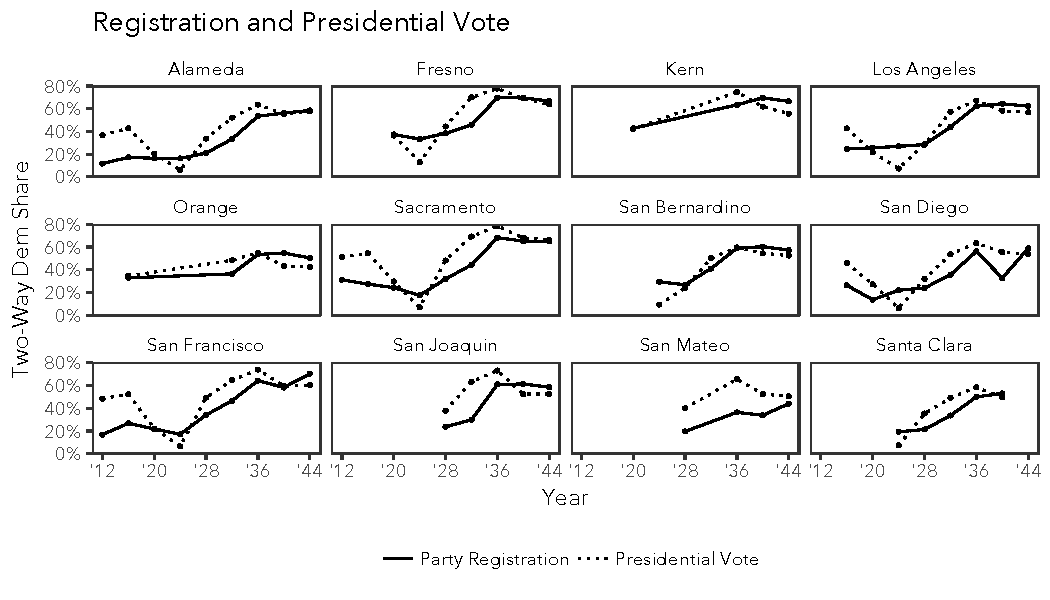
\includegraphics[width=\maxwidth]{figures/plots-countyparty-1} 

}

\caption[Two-Way Democratic presidential vote share and Two-Way Democratic Registration share by year]{Two-Way Democratic presidential vote share and Two-Way Democratic Registration share by year. Due to issues extracting data from the Great Registers, not every county has registration data for every year. For clarity, when data from the Great Registers is missing, data on presidential vote for that county-year pair is also excluded. Only counties that had Great Register data before 1930 and after 1936 were included in this plot.}\label{fig:countyparty}
\end{figure}


\end{knitrout}

\FloatBarrier
\subsection*{Is California a representative case?}

Even if one accepts that the Great Registers provide a reasonable picture of Californians' partisan attachments, the connection between California politics and those of America broadly is still up for debate. Even in 1910, California was home to nearly 2.4 million people, a population that more than quadrupled by 1950. The political behavior of these Americans should itself be of interest.  But if these Californians are reasonable proxies for the behavior of their eastern compatriots, a broader and more important story can be told.  

One set of states that California should not be compared to is the South. Southern states did not realign toward the Republicans in 1894, instead remaining consistently supportive of the Southern Democratic party, in contrast to Republican dominance in California. Southern voters also had lower rates of turnout. The voter turnout rate was only about a quarter in the Southern states, compared to just under half for the rest of the country \citep{burnham1965changing}.

Counties are the lowest geographic unit for which election data is consistently available for the early twentieth century, and at this level voting in California looked broadly similar to the rest of the non-Southern states.  Figure~\ref{fig:countydensity} shows the distribution of county-level presidential vote for 1912-1940 in California and in other non-Southern states. Except in 1924, when Progressive presidential candidate Robert La Folette was popular among historically-Democratic rural voters in California, the distribution of county-level Democratic presidential vote was near the median of the distribution of the same measure in non-Southern states. One other way that California is unrepresentative is that in 1912, Taft did not appear on the ballot. Instead, voters chose between Wilson, running as a Democrat and Theodore Roosevelt, running under the Progressive banner.

Returning to the Literary Digest polls discussed in the introduction, we can evaluate not just presidential vote, but also vote-switching, an important theme of this paper. Californians had rates of political defection about as high as voters in non-Southern states overall. Among Californians, 52\% of Davis voters switched to Hoover in 1928, while 26\% switched from Coolidge to Smith.  The comparable national numbers were 35\% and 23\%, respectively. The rate of defection among Californians is higher than among voters nation-wide, but both shared a rate of vote-switching much higher than typical in modern elections.




\begin{knitrout}
\definecolor{shadecolor}{rgb}{0.969, 0.969, 0.969}\color{fgcolor}\begin{figure}

{\centering 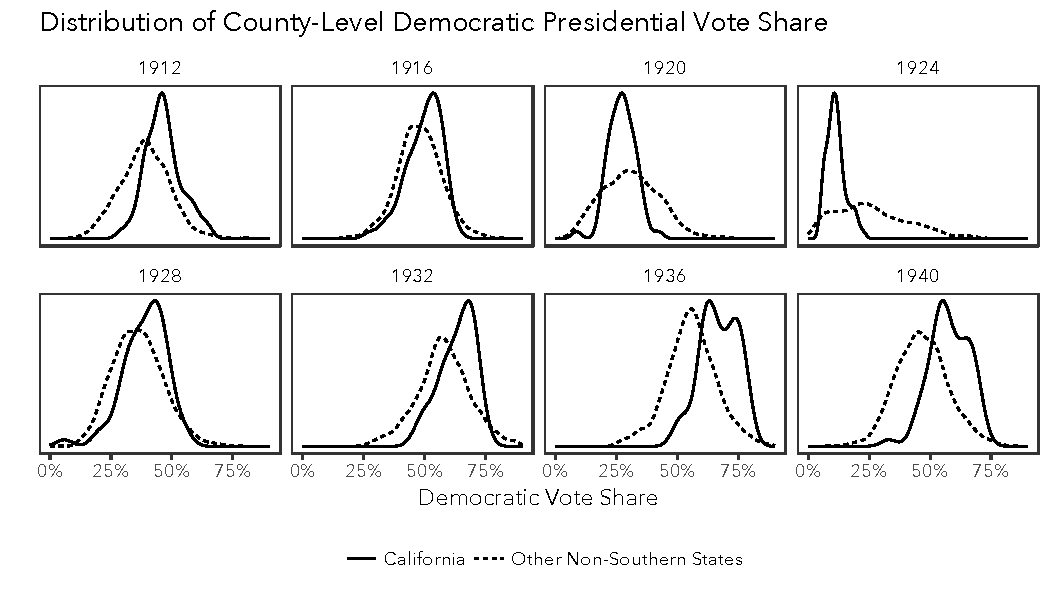
\includegraphics[width=\maxwidth]{figures/plots-countydensity-1} 

}

\caption[Density plots of county-level presidential vote share for California (the solid line) and counties in non-Southern states (dashed line) for presidential elections 1912-1940]{Density plots of county-level presidential vote share for California (the solid line) and counties in non-Southern states (dashed line) for presidential elections 1912-1940. For the purposes of this analysis, Alabama,	Arkansas,	Florida,	Georgia,	Kentucky,	Louisiana,	Mississippi,	North Carolina,	South Carolina,	Tennessee,	Texas,	Virginia and	West Virginia were removed.}\label{fig:countydensity}
\end{figure}


\end{knitrout}



\subsection*{Two-Party Consolidation}

Looking at election results before the New Deal, the influence of the Progressive party is unmistakable. Hiram Johnson was elected governor of California as a Republican in 1910, but went on to co-found the Progressive party with Theodore Roosevelt in 1912, serving as its Vice-Presidential nominee in that year.  When Johnson ran for re-election as governor in 1914, the Progressive party made huge gains in voter registration, taking about a quarter of Republican registrants and making them, for a time, Progressives.

Figure~\ref{fig:consolidation} shows that this swell of Progressive affiliation did not last, however.  The Progressives did not field a candidate in the 1918 gubernatorial election, and over time, the party lost nearly all of its registrants.  Though the Socialist and Prohibition parties never received the ground-swell of support that the Progressives received in 1912 and 1914, they too saw their numbers decline to a negligible level by 1920.  By 1922, the rate of voters declining to affiliate with a major party also declined, leading to an increasing proportion of voters registering with the two parties.  By 1930, the last year before the New Deal realignment took place in California, 93\% of voters were registered with one of the two major parties, a rate that declined further in the coming years.

\begin{knitrout}
\definecolor{shadecolor}{rgb}{0.969, 0.969, 0.969}\color{fgcolor}\begin{figure}

{\centering 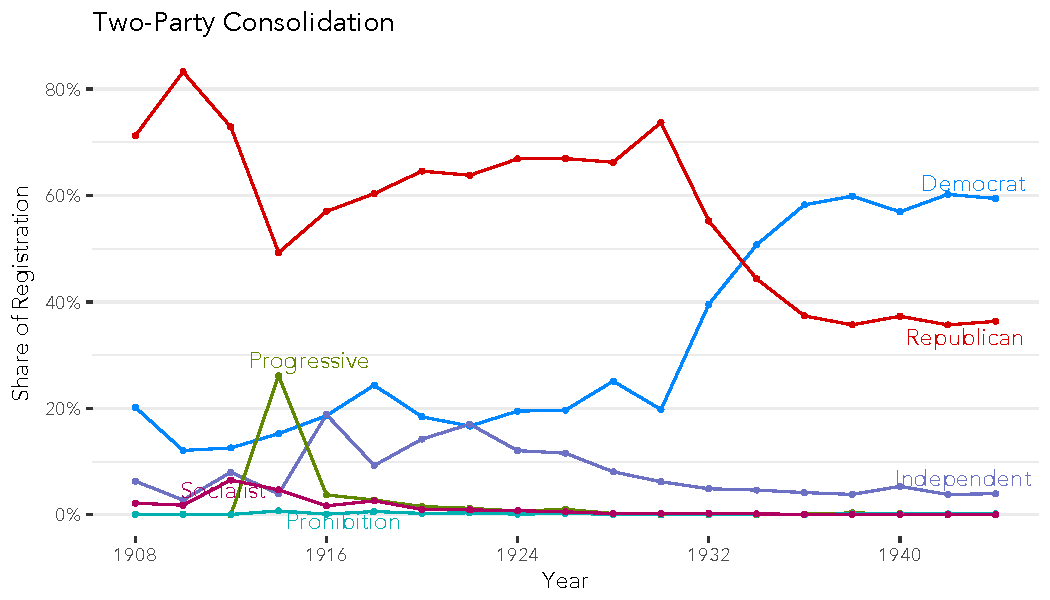
\includegraphics[width=\maxwidth]{figures/plots-consolidation-1} 

}

\caption[Rates of party registration for the six most common parties, 1908-1944]{Rates of party registration for the six most common parties, 1908-1944.}\label{fig:consolidation}
\end{figure}


\end{knitrout}

The high proportion of voters that registered with the two parties is helpful for measuring partisan sentiments.  On the 2013 California voter file, only 72\% of Californias registered with one of the two major parties. Many of the remaining voters themselves held strong partisan preferences toward one party or the other, but this preference is unknowable from voter file data alone. Luckily, many more voters on the Great Registers are affiliated with a party.  Except for 1914, when the shift in party registrations to the Progressives led 30\% of California voters to be affiliated with the Progressive party, the two major parties' share of registrations never dipped below 75\%.  By 1928, the last presidential election before the realignment, just 10\% of the electorate wasn't registered with one of the two parties.

The increasing dominance by the two major parties was an important precursor to the realignment, as it reduced the opportunity for competition outside the two party system.  It is impossible to know what would have happened had the Great Depression struck in 1912, as Theodore Roosevelt mounted a run for the White House under the progressive banner. Perhaps the Progressives would have made huge gains and formed a new party.  But by 1932, there was only a single organized alternative to the Republicans. 

In 1932, President Hoover received a letter from an Illinois voter, "Vote for Roosevelt and make it unanimous." The Democrats took power amidst popular disapproval of Hoover's efforts to reverse the effects of the Depression. They were the recepients of vast numbers of new registrations and twenty years of continuous control of the White House. In this way, the narrower set of choices available to voters all but guaranteed that if voters were to leave the Republicans en masse, as they did in the 1930's, they defected to the Democrats, the only other party with a significant number of registrants.


% are independents just an intermediate category?
% Look at how big a share progressives got: shows prima facie that party attachments are weak


\section*{Party Switching}


%%% show that panel data partisanship looks like overall partisanship

That partisanship is stable and central to a voter's political attitudes has been fundamental to the study of American political behavior since the publication of the \emph{The American Voter} in 1960. The simple descriptive fact that voters tend to form a party affiliation early in their lives and retain it for many years has been measured repeatedly and confirmed to be a consistent feature of American public opinion since the 1950's \citep{green1994stable, clarke2009dynamics}. 

Though the Literary Digest Straw Polls suggest that presidential vote choice was more fluid before the New Deal realignment, no direct evidence on partisanship is available from survey data before 1936. This makes the Great Registers the only viable way to test whether partisanship was stable during the fourth party system, as it is in the fifth. On this point, the Registers are clear. It was not.

Before 1928, the Democratic party, already small, hemoraged an average of 23\% of their voters to the Republicans each election cycle. Figure~\ref{fig:pid_switching} shows the rates at which each party lost their members to the opposing party in successive presidential election years from 1908 to 1960, among members registered with the two parties in both elections. The Democratic party held on to a relatively small proportion of its members through this period, losing around  20\% of its membership to the Republicans in each year from 1908 to 1924 (meaning they appeared as members of the other party from 1912 to 1928). Despite the fact that Democrats had already incurred huge losses in the 1896 realignment, the party continued to lose members until the New Deal realignment began in 1932.  The only reason the Democratic party membership did not shrink further is that these relatively large losses by Democrats were offset by proportionally smaller losses from the Republicans. Because the Republicans had a much larger base to begin with, the Republicans could lose an average of just 5.5\% of their voters to the Democrats each year and have those losses offset by defecting Democrats, who on two occasions lost more than 30\% of their members in a single presidential election cycle.


\begin{knitrout}
\definecolor{shadecolor}{rgb}{0.969, 0.969, 0.969}\color{fgcolor}\begin{figure}

{\centering 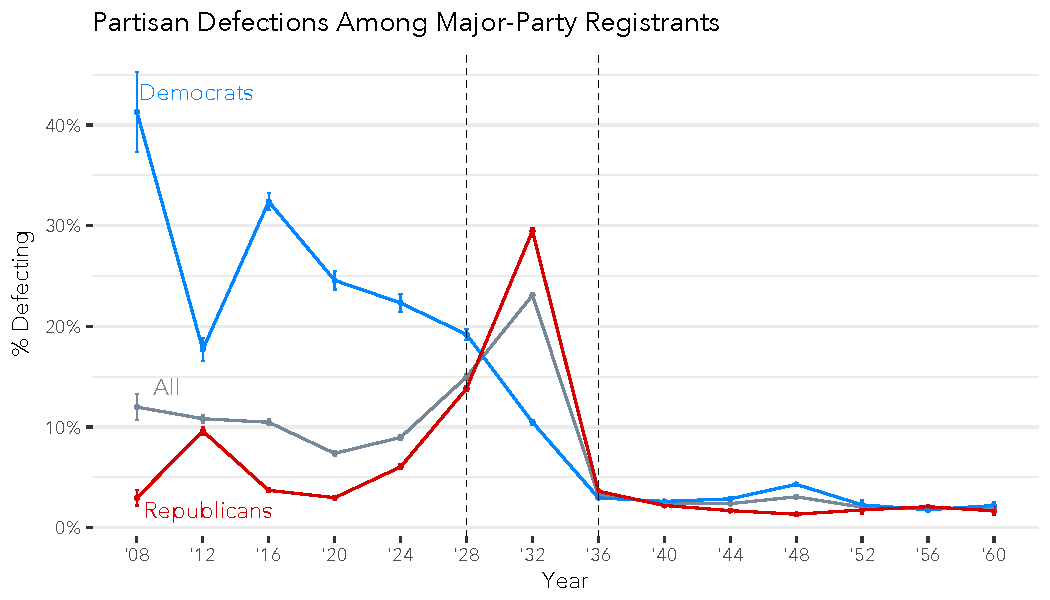
\includegraphics[width=\maxwidth]{figures/plots-pid_switching-1} 

}

\caption[Rates of party switching between successive presidential elections among voters registered with the two major parties in both elections]{Rates of party switching between successive presidential elections among voters registered with the two major parties in both elections. The figure was generated by matching records appearing in successive presidential years that share an address, surname, and first name. This stringent requirement for matching excludes movers and records with transcription errors, but keeps false matches, which inflate the rate of party-switching, to a minimum. Frequentist 95\% confidence intervals are plotted as vertical lines.}\label{fig:pid_switching}
\end{figure}


\end{knitrout}
 
\FloatBarrier
This pattern of partisan churn implies something extraordinary about the composition of the Democratic party during the pre-realignment period: a significant proportion of Democrats had recently been Republicans. Figure~\ref{fig:party_composition} shows that in 1916, nearly 30\% of Democrats were registered Republicans four years prior. Political scientists have come to view parties as coalitions of voters, led by political elites, that compete for votes. But if these elites are leading an ever-shifting group of voters, as many as 30\% of whom were recently registered with the opposing party, this model cannot describe partisan competition in the mass public. 

This disconnect between the partisanship of office-holders, who rarely switched between the two major parties, and voters, who did so frequently, might be explained by the kinds of issues contested in the fourth party system. Aside from prohibition and women's enfranchisement, two issues which drew much fervor but were not polarized along partisan lines, many of the partisan issues of the day were technocratic in nature. Debates about how to handle railroad and industrial trusts, the proper levels of tariffs, the banking system and the gold standard were quite disconnected from the lives of most Americans, particularly relative to the politics of the New Deal, which focused on jobs and public assistance programs during the Depression. As the issues attached to the two parties' platforms became more salient to voters, their attachments stabilized, and the weak attachments of the fourth party system gave way to the strong partisan ties of the fifth party system, which remain today.



\begin{knitrout}
\definecolor{shadecolor}{rgb}{0.969, 0.969, 0.969}\color{fgcolor}\begin{figure}

{\centering 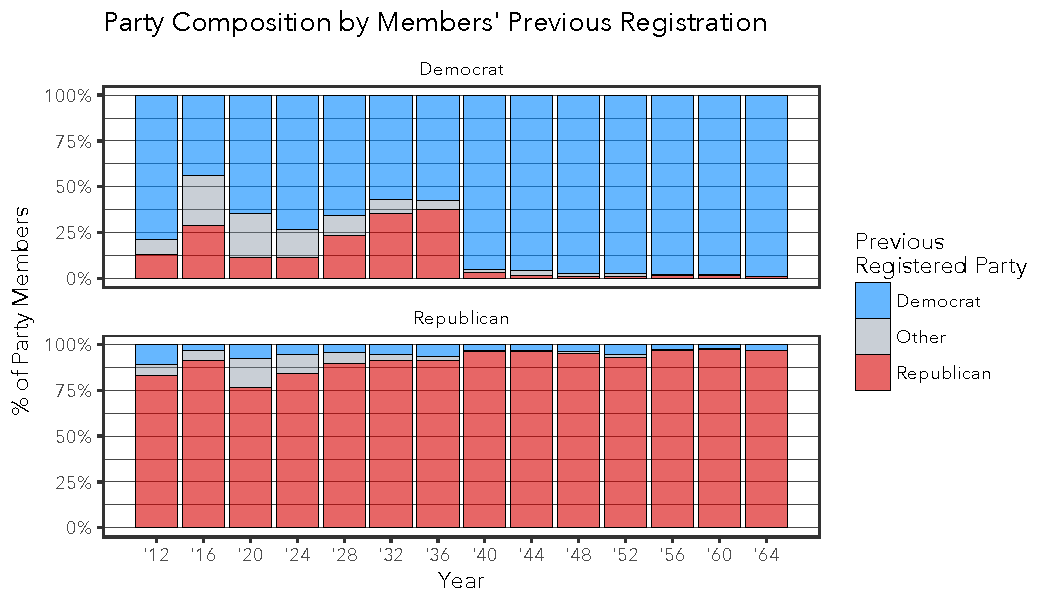
\includegraphics[width=\maxwidth]{figures/plots-party_composition-1} 

}

\caption[Composition of the two major parties by members' party registration in the previous presidential election]{Composition of the two major parties by members' party registration in the previous presidential election. Members not found on the rolls for the previous election are excluded from the figure.}\label{fig:party_composition}
\end{figure}


\end{knitrout}
 

The high level of churn in both parties, but especially among the Democrats, must have posed tremendous challenges for party governance. How could party elites form a stable hold over their state parties if so much of the membership turned over every four years? For Democrats before 1936, at least 12.5\% of their members were recently Republicans in each election year, and nearly 25\% of their members were previously Republicans or not registered with a major party in the last election (this doesn't count those members who were not registered at all). One possibility is that primary voters were loyal to their party, while the voters most likely to switch parties did not vote in primaries.  Without turnout data, this is impossible to know, but it seems that a full account of how parties operate during the period must account for the transience in the Democrats' ranks. The GOP's membership was more stable, but the party rolls were filled with fewer stable Republicans than after the realignment, when both parties membership rolls stabilized at less than 5\% churn per year.


In 1932, this Republican-favoring equilibrium broke and a huge number of voters left the Republican party for the Democrats. Democrats became modestly better at holding on to their voters, while Republicans became substantially worse at holding on to theirs.  Though Democrats were holding on to more of their voters than they had in the first three decades of the century, many Democrats were still defecting to the GOP, indicating that the realignment was not entirely one-sided. As the realignment wore on, Democrats lost about 10\% of their voters in each election, but Republicans grew worse at holding on to their voters. 30\% of Republican voters in 1932 became Democrats by 1936.   

Then, in 1936, the party ledgers nearly froze. From 1936 forward, each party held on to over 97\% of their voters. Now that voters from both parties had stable attachments to their party, the notion that party identification was the central component of attitude-formation for partisans finally seems to be a plausible.

\subsection*{Proposition 14}

Survey data collected after the New Deal realignment suggests that we should see a low level of inter-party defections after the New Deal. This pattern is unambiguous in the Great Registers, only about 2.5\% of registrants change their party registration from one presidential election to the next. The correspondence between these results shows that behaviors observed on the Great Registers match survey results, thereby increasing the credibility of the Great Registers as a research tool. It also makes the volatility of the pre-realignment period more striking; the volatility of the first three decades of the twentieth century is totally out of line with the partisan stability of the post-realignment period.

The passage of Proposition 14 in 1930 changes the interpretation of the post-1932 data. The measure amended the statute governing voter registration, requiring the state to maintain registrations from the previous two-year election cycle and allow the previous cycle's voters to vote in the next cycle without re-registering. This meant that voters that voted consistently would not  need to file a new registration nor update their occupation or party registration. Non-voters, however, would be removed from the rolls and sent a postcard alerting them that they had to re-register in order to vote in the next election. About 20\% of registered voters didn't vote in presidential general elections and 25-40\% didn't vote in midterms, so many voters did have to file new registrations each year, in addition to those that had to re-register due to a change in residence. 

These re-registrants are key to creating a set of voters who made updates to their voter registration, just as all registrants did before 1934. Among the set of registrants matched to their own registration from four years later in figure~\ref{fig:pid_switching}, I want to identify those that were not registered in the midterm election, indicating that they had to re-register in advance of the next presidential election. The matching method used for the figure~\ref{fig:pid_switching} panel was quite conservative, only making matches when the match was nearly certain. This restriction surely missed many correct matches, but it kept the false positive rate to a minumum, thereby minimizing the bias toward a higher rate of defections created by erroneous matches. To identify registrants missing from the midterm election rolls, a more relaxed match method is necessary. Such a match method should, to the extent possible, minimize the false negative rate, so that panelists that might not have had to re-register can be excluded.  The goal is to find a subset of panelists that would have had to re-register. The party switching rates for new and continuing registrations are plotted in figure~\ref{fig:prop14}. Among the 10\% of presidential-election registrants for which no midterm registration appeared, the party-switching rate averaged just 3\% and never exceeded 5\%, indicating that party-switching had indeed fallen from the 10\% rate observed before the realignment.


\begin{knitrout}
\definecolor{shadecolor}{rgb}{0.969, 0.969, 0.969}\color{fgcolor}\begin{figure}

{\centering 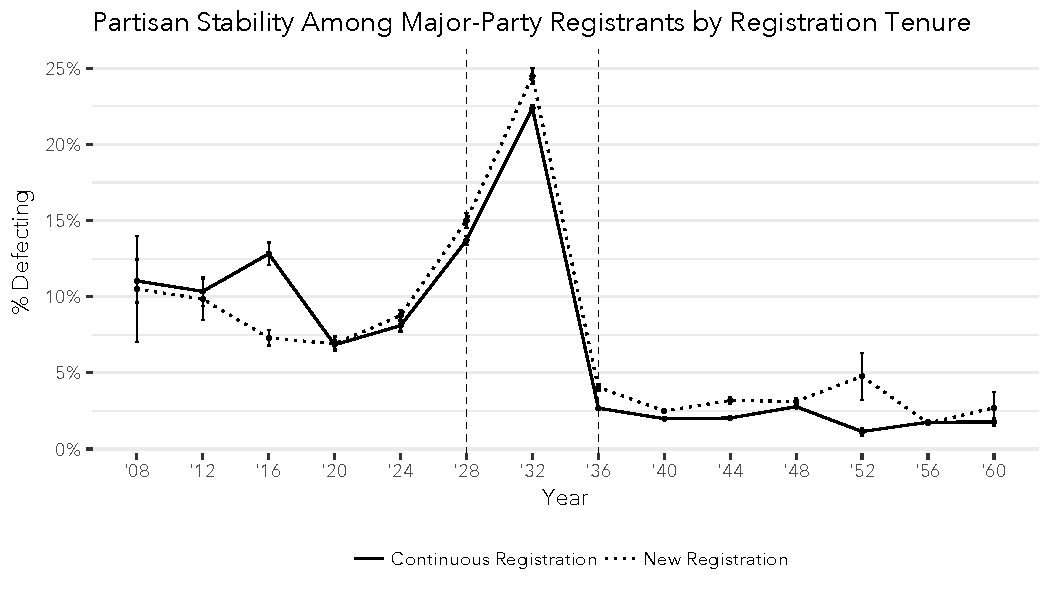
\includegraphics[width=\maxwidth]{figures/plots-prop14-1} 

}

\caption[Rates of party switching between successive presidential elections among voters registered with the two major parties in both elections]{Rates of party switching between successive presidential elections among voters registered with the two major parties in both elections. The figure was generated by matching records appearing in successive presidential years that share an address, surname, and first name (using the corrected first and last names discussed earlier). Records for which no registration in the midterm election was found are classified as having a new registration, while voters that were registered in the midterm are classified as having a continuous registration. For the purposes of matching a midterm registration, a loose match method was used, leading to many new registrations to be falsely classified as continuing. Frequentist 95\% confidence intervals are plotted as vertical lines.}\label{fig:prop14}
\end{figure}


\end{knitrout}


\section*{Voting in Groups}

The notion that voters have many intersecting social identities that characterize their partisanship is central to the study of public opinion and political history. That divisions among voters along racial, ethnic and generational cleavages would also lead to divisions in their partisanship is a core tenet of descriptive work in American public opinion \citep{berelson1954voting}. Sundquist \citeyearpar{sundquiest1983dynamic} goes even further, "The behavior of individuals cannot be analtzed or discussed  until they are grouped in some manner; there are just too many of them." But before the advent of public opinion polling, systematic evidence of the kind now common in the field of public opinion was  unavailable.  The Great Registers offer the first representative individual-level data of demographic partisan cleavages before 1936.

Without detailed micro-level data, it is natural to characterize the divisions of the past using the analytical tools of the present. Much of Andersen's \citeyearpar{andersen1979creation} characterization of the politics of the pre-realignment period is driven by the assumption that individual partisanship is stable and that age, class and ethnic cleavages analogous to the post-realignment period were present in the electorate, but only revealed later with scientific polling. But just as individual-level data from the Great Registers has shown that partisan stability was much lower in the period before the New Deal, so too were partisan divisions between groups less pronounced.

Public Opinion before 1936 was nothing like public opinion of the post-realignment period. Not only was the public altogether more Republican, but many dimensions of social difference showed little or no partisan differentiation at all. Before the realignment, low-skilled blue collar workers were just 4 percentage points more Democratic than white collar workers. After the realignment, this cleavage grew to 25 p.p. An age gap in partisanship also emerged: there was no difference in the partisanship of the youngest and oldest voters before 1932, but after, the youngest Californians were 10 percentage points more Democratic that the oldest voters. Even in national origin, a common way to discuss social divisions in the early twentieth century, the differences between ethnic groups' average partisanship grew by a third. In the context of low political participation, low levels of inter-party competition and abstract issues before the congress, there was less reason to mobilize members of one's social group for a particular party \citep{burnham1965changing}.

The observation that public opinion is driven by group identities is not new, but it has received new attention recently, as Achen \& Bartels \citeyearpar{achen2016democracy} have argued that group identities are the best framwwork with which to understand individuals' political choices.  This is surely a useful framework for thinking about the present, but the social groupings of the pre-Realignment era did much less explanatory work before the New Deal.

\subsection*{Class}

% footnote about women
% white collars also realign

The coalescing of the American party system around competition between a party representing the interests of capital (the Republicans) and the party of labor (the Democrats) is one of the defining facts of the New Deal Realignment. Lipset \& Rokkan \citeyearpar{lipset1967cleavage} document this trend in several Western countries, observing that the social divisions of the 1920's were expressed in the agendas of political parties and frozen in place in what appeared to be permanent political divisions. The context for this so-called \textit{freezing hypothesis} is important, as it tells us about the pre-conditions for permanent class cleavages to take hold.  Lipset \& Rokkan's argument applies to advanced democracies broadly, but the American transition from the fourth to the fifth party system can serve as an interesting study of how this freezing took place.

It might not be mere coincidence that that the freezing of partisan identities  and the freezing of the core cleavage defining the (non-Southern) American party system both occured in 1936.  Before the New Deal realignment, party registration was fluid, so large changes in the issue orientation of the parties could be bolstered by a large pool of loosely attached voters that could rally behind the party's new platform.  This is surely what happened during the New Deal realignment, which led voters from across the social classes to coalesce and solidify behind the Democrats. These voters, once captured by the Democratic party or by the Republicans, stayed, and the issue orientation of the parties solidified.  Would the parties have been able to hold on to their newly-loyal voters if they changed their core platforms? Perhaps so, but in the context of two nationally competitive parties with stable bases, elites that sought to change the orientation of the party could not rely on an influx of new party members to bolster reform against pressure from incumbent members invested in the status quo. In the context of loyal partisans, a change in issue orientation may have been too risky for parties committed to maintaining incumbents' hold on power.


\begin{knitrout}
\definecolor{shadecolor}{rgb}{0.969, 0.969, 0.969}\color{fgcolor}\begin{figure}

{\centering 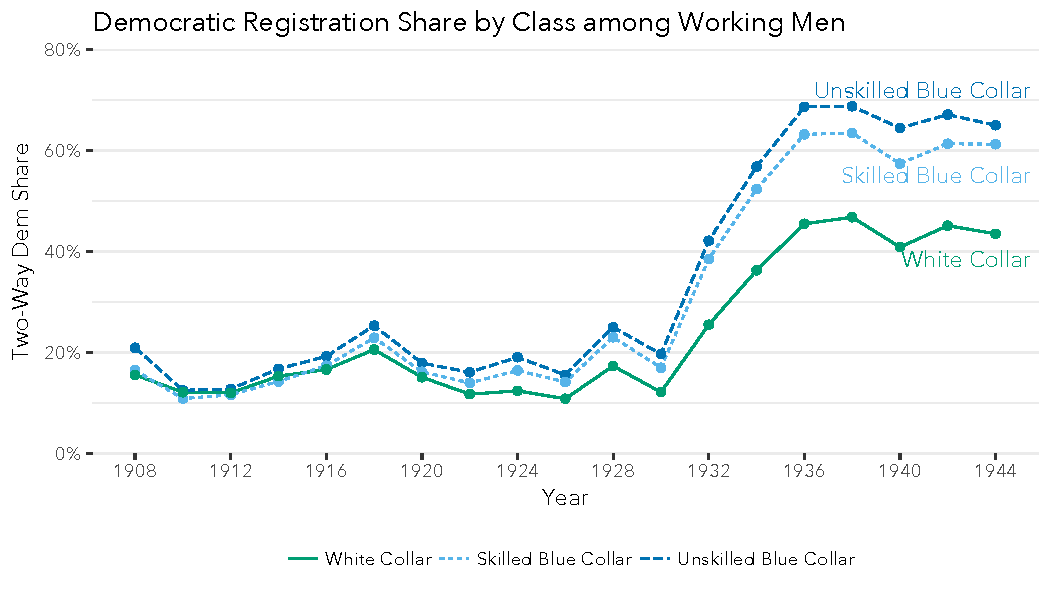
\includegraphics[width=\maxwidth]{figures/plots-class-1} 

}

\caption[Rates of Democratic partisan identification by class among men identifying with the 400 most common occupations, classified into the three class categories]{Rates of Democratic partisan identification by class among men identifying with the 400 most common occupations, classified into the three class categories.}\label{fig:class}
\end{figure}


\end{knitrout}

Before 1932, and particularly before 1918, the relationship between social class and partisanship was remarkably weak. There was virtually no absolute difference in the partisanship of people of different social classes. After at least 22 years of partisan competition not organized along class lines, a class cleavaged emerged rapidly in the New Deal realignment. As the overall level of Democratic party identification increased rapidly, figure~\ref{fig:class} shows how the absolute difference in party identification rates diverged.  In 1930, the difference in partisanship between unskilled blue collar workers and white collar workers grew to 7 points, a gap already larger than it had been earlier in the fourth party system. Just six years later, the gap had more than tripled, with about 69\% of unskilled blue-collar workers registering with the Democrats, compared to 46\% for white-collar men.

It's clear that by 1936, unskilled blue collar workers were much more likely to identify with the Democrats than higher-skilled (and presumably higher-paid) voters. But the rates of Democratic party identification among white-collar workers also increased, leaving the relative levels of Democratic registration unchanged. The class composition of both major parties remained nearly constant, even though there was a large aggregate move from the Republicans to the Democrats. The same pattern holds at the level of occupations, an occupations partisan composition in 1930 explains 60\% of the variance in the occupation's composition in 1940, with the average occupation increasing in the proportion of Democrats by 133\%.




\FloatBarrier
\begin{knitrout}
\definecolor{shadecolor}{rgb}{0.969, 0.969, 0.969}\color{fgcolor}\begin{figure}

{\centering 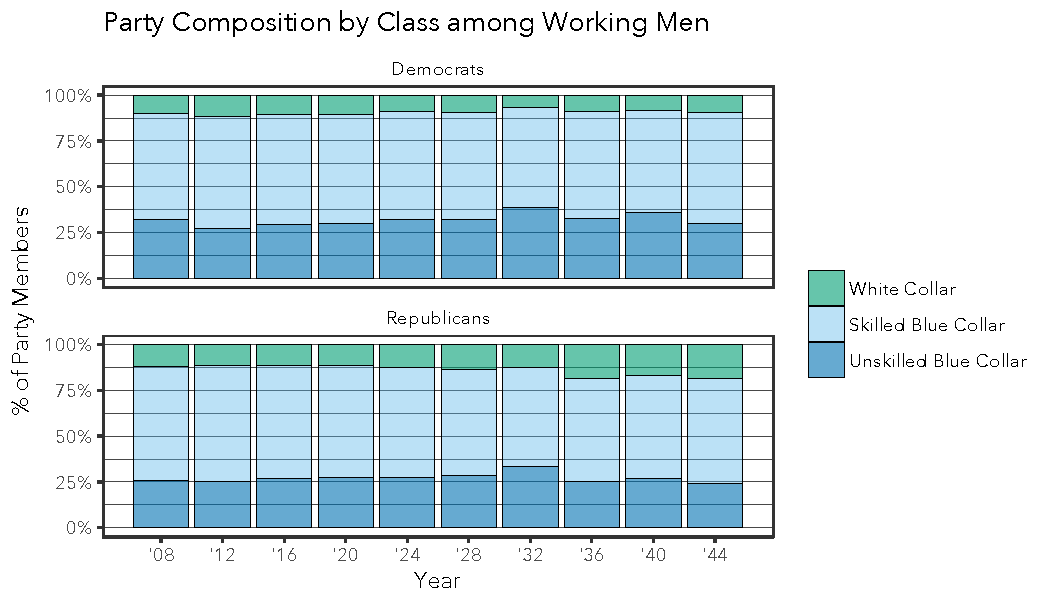
\includegraphics[width=\maxwidth]{figures/plots-class_composition-1} 

}

\caption[The proportion of each party from each socio economic class is shown above]{The proportion of each party from each socio economic class is shown above. The class composition of both parties remained essentially constant over time, even as huge numbers of voters flocked to the Democrats.}\label{fig:class_composition}
\end{figure}


\end{knitrout}


The stability of the class composition of the parties is shown in figure~\ref{fig:class_composition}. Other than a slight decrease in the proportion of skilled blue-collar occupations and a slight increase in the proportion of white-collar workers, the class-composition of the Republican party was quite stable. The Democratic coalition was even more stable, showing fluctuations in the party composition over time, but no secular changes.  Remarkably, the composition of the two parties were quite similar to each other: Republicans had a marginally higher status coalition than Democrats both before and after the realignment. 

Though the New Deal period brought large changes in the platform of the two parties, with Democrats championing government intervention into the economy in the form of the New Deal programs, the actual socio-economic composition of the parties did not change.  Extrapolating from two descriptive facts about the New Deal--- the increasing proportion of working-class voters identifying as Democrats and the new more left-wing platform of the Democratic party--- scholars understandably concluded that the New Deal coalition was different in character than the Democratic coalition that preceded it.  In some sense, this is true. Millions of new voters joined the Democratic coalition, expanding its ranks dramatically. This swell gave the Democrats vastly more political power, making the New Deal reforms possible. But simply because the parties ranks had swelled, it does not mean that they were drawing their members from new groups or that the character of its membership had changed. Instead, the same types of voters that had supported the party since 1918 drove its rise under Roosevelt. 

This type of error is an understandable consequence of thinking about politics in terms of groups. Democrats went from losing blue collar workers 4-to-1 to winning a comfortable majority of blue-collar workers.  At the same time, Republicans held on to most white-collar workers, keeping a majority of those registered with the Republican party. From this type of statement, it is tempting to conclude that Republicans were the party of the rich and Democrats the party of the working-class, but this is simply not the case. In both parties, the median voter was solidly blue-collar.  Indeed, given the class makeup of the country, no other configuration was possible.

\subsection*{Birth Cohort}

The notion that different generations have distinctive politics is commonplace in political science. Voters of different generations are socialized into politics during different political periods, and are usually thought to have unique partisan attachments that make them different from younger or older voters, who came of age in a different political moment \citep{klecka1971applying}. This model of politics is undergirded by two stylized facts: that early partisan socialization is important and that partisanship is mostly stable over-time. The first idea is that events early in one's life have more influence over political attitudes than events that occur long after the voter has become politically active \citep{sears1997politics,bartels2014generational,ghitza2014great}. The second element is that once socialized, the high degree of partisan stability observed in American public opinion will preserve the effects of this early socialization for decades to come. But in the context of low partisan stability in the early twentieth century, the effects of early socialization did not persist later in life. In fact, partisan instability was so extreme that it created virtual uniformity across age cohorts before the realignment. 

\begin{knitrout}
\definecolor{shadecolor}{rgb}{0.969, 0.969, 0.969}\color{fgcolor}\begin{figure}

{\centering 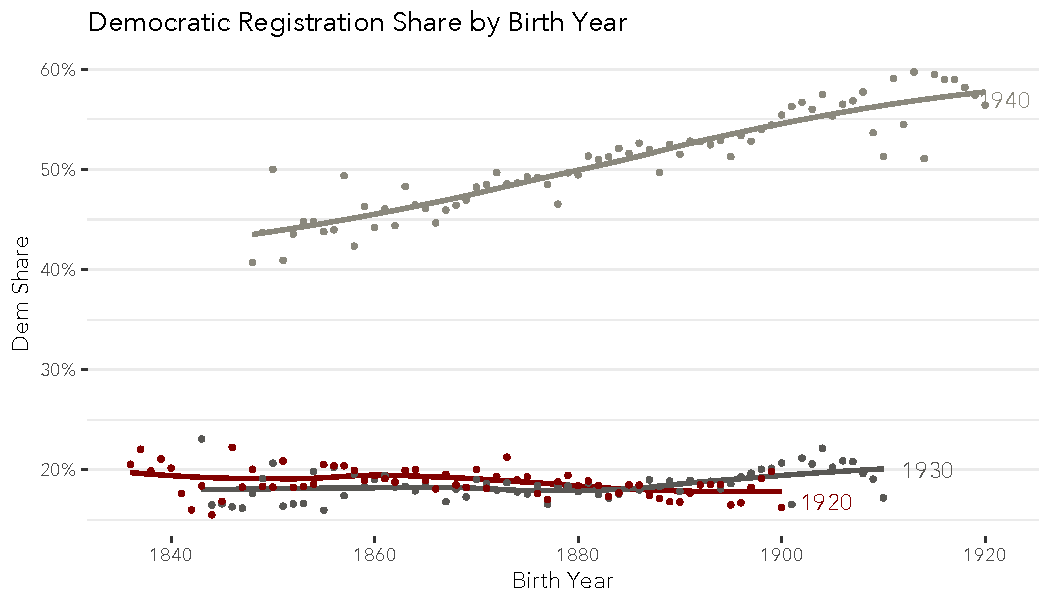
\includegraphics[width=\maxwidth]{figures/plots-age-1} 

}

\caption[Rates of Democratic partisan identification by the voter's year of birth (inferred from their age)]{Rates of Democratic partisan identification by the voter's year of birth (inferred from their age). Age is drawn from the 1920, 1930 and 1940 Censuses, matched to the Great Registers of the same year with exact matching on name and street. Age categories with fewer than 100 people were excluded. The lines represent loess fits to the aggregated data.}\label{fig:age}
\end{figure}


\end{knitrout}

This uniformity is clear in figure~\ref{fig:age}. In 1920 and 1930, voters across birth age cohorts were about 15 to 20\% Democratic. This uniformity is surprising, given that voters that came of age before the 1894-1896 realignment would have started voting in a period where California was more supportive of Democratic candidates than they were from 1896-1932, when Republicans and Progressives dominated state politics. Andersen \citeyearpar{andersen1979creation} has suggested that voters that came of age during a realignment, when partisan fervor is most titled toward one side, should be especially supportive of the ascendant party. But by 1920, no distinctiveness of the 1896 realigning generation remained.  It would seem that the partisan instability that characterized the period wiped away any gains Democrats would have made.  Conversely, socialization theory would suggest that voters born around 1876, who would have come of age just as the 1896 realignment was taking place, would be more supportive of Republicans. Though this group supports Republicans over Democrats by a 4-to-1 margin, they are not unusually Republican, as socialziation theory would have us expect. 

After the New Deal realignment, age cohorts were significantly more differentiated. There is essentially a linear relationship between age and Democratic registration, suggesting that socialization theory works as predicted. The youngest voters, who came of political age during the depression and the Roosevelt administration, were most supportive of Democrats, while the oldest voters were more likely to stay with the Republicans. Despite the thrend of older voters being more Republican than their younger counterparts, even the most elderly voters, who were as old as 90 when the 1940 election took place, were 25 percentage points more Democratic than they had been ten or twenty years earlier.  This dramatic shift shows the power of the realignment in changing the attitudes of even those voters one would expect to be most likely to stay with the Republicans.


\subsection*{National Origin}


In the absence of clear individual-level partisanship data, it is often convenient to discuss partisanship in terms of geographically concentrated groups. Because people of common national origin tend to concentrate geographically and share cultural traditions, it is natural to talk about ethnic groups as salient to political competition. Lubell \citeyearpar{lubell1952future} believed that the influx of immigrants in the early twentieth century had made a large partisan change inevitable. Whether one believes the realignment was destiny, it does not  follow that immmigrants had distinctive political attachments before or after the realignment.

Compared to today, when African-Americans and hispanics are substantially more likely to vote for Democrats than  whites, the race and ethnic divisions of the time were small.  In both 1930 and 1940, the partisanship of African-Americans nearly exactly matched that of whites. This suggests that there was no racial cleavage for the black population, which made up around 1.5\% of the state's voters. 

Among immigrants and their children, there was at best a modest relationship between ethnic origin before the realignment.  Figure~\ref{fig:natl_origin} shows the relationship by father's national origin between parisanship in 1930 and 1940. In 1930, the standard deviation of the two-way Democratic registration share (the horizontal variation) was 6.7\%. After the realignment, this variation (the vertical varation in figure~\ref{fig:natl_origin}) increased by a third, to 9.2\%.  Though there was certainly some variation explained by immigrant group, the variation explained is small.  In 1930, 18\% of Californians with native fathers were Democrats. On average, 18\% of Californians with foreign-born fathers were also Democrats. Indeed, with the exception of a few ethnic groups, most ethnic groups were also near the 18\% average. After the realignment, first and second-generation immigrants were 5 percantage points more Democratic. In 2013, second-generation hispanic immigrants were 23 percengate points more Democratic than the American public generally, while Asians were six points more Democratic. Thus, the small nativity gap of the pre-New Deal period is anomolous both by the standards of post-realignment politics and of today.

\begin{knitrout}
\definecolor{shadecolor}{rgb}{0.969, 0.969, 0.969}\color{fgcolor}\begin{figure}

{\centering 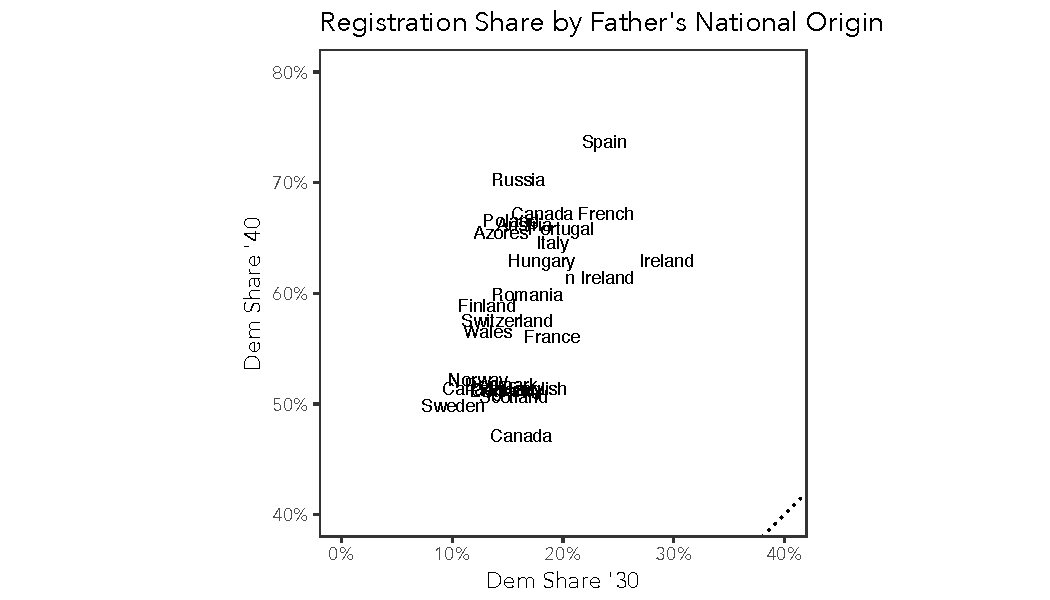
\includegraphics[width=\maxwidth]{figures/plots-natl_origin-1} 

}

\caption[This figure shows the proportion of people registered with the Democratic party by father's place of birth]{This figure shows the proportion of people registered with the Democratic party by father's place of birth. As usual, the proportion is calculated with respect to voters registered with one of the two major parties.}\label{fig:natl_origin}
\end{figure}


\end{knitrout}

The partisanship of immigrants before the New Deal is not merely important as a description of public opinion before the New Deal, it also provides important context for understanding the mobilization account of the realignment. In the mobilization story, much of the increase in Democratic votes during the realignment comes from the mobilization of immigrants and their children. But if the mobilization account is to be believed, these immigrants and their children must already have been Democrats (or disposed to become Democrats) and simply were not voting. We cannot know the party registrations of people that weren't registered to vote, but it stands to reason that those first and second-generation immigrants that were registered to vote were politically similar to those that were not.  If this was the case, then the unregistered population was about as Democratic as those that were registered to vote, making the mobilization account implausible.

\section*{Conclusion}

% move from flip-flop to stable
% 

The tools of public opinion research were developed in an age of structured and stable party affiliations. Individuals were loyal to their parties and social groupings had different partisan attachments. But before the realignment, mass partisanship was descriptively quite different. 10\% of voters switched parties every four years, and social markers like age, race and national origin explained far less of the individual variation in partisanship than in later years. This meant that even in homophillic social networks, individuals would have known Democrats and Republicans in roughly equal proportion to the general population. This distinct period of political history occured just before the New Deal realignment, perhaps the most consequential time for mass politics in the twentieth century. Understanding the period from 1910 to 1930 sheds new light on the realignment and helps contextualize the differing accounts for how the realignment took place. In light of what we know about the strong and remarkably uniform support of the Republican party, mass partisan conversion of Republicans into Democrats seems to be the only plausible source for Democrats' new support. There simply were not pockets of Democrats waiting to be mobilized.

That the distinctive character of politics before the realignment went undiscovered for nearly 90 years is no surprise; the research tools to conduct this analysis simply did not exist. The research tools simply did not exist. In the early years of the ANES, respondents' self-reported turnout was validated against county voting records. But this validation was eventually abandoned as too difficult for interviewers. Without the benefit of contemporary optical-character recognition and data-management software, research assistants would have to cross-reference individual voters within bound voter lists, later finding these same voters in paper census records. It's hard to estimate how proficient research assistants could be trained for this task, but the benefits of modern technology are clear.  To study this period before surveys, computing power tied to suitable administrative records is the best means of gathering individual data.

These records overturn many would-be laws of American public opinion. Research on realignments conceives of partisanship as generally static, punctuated by periods of rapid change. But before the New Deal, individual change was constant, even as macropolitics were in a stable Republican-dominated equilibrium. When the earliest entries into the canon of American political behavior were written in the 1950's, America had enjoyed a relatively stable two decades of partisan competition. Voters had stable party affiliations that flowed in part from their membership in social groups. Had the survey-based architecture of American public opinion formed twenty years earlier, very different accounts of American political behavior would have been written. Partisan stability would be treated not as an essential element of the American political mind, but instead as a historically contingent phenomenon emerging out of the tumult of the 1930's. Given the picture of partisanship offered by the Great Registers, we now know that the cast of \textit{The American Voter} was forged in 1936.




\clearpage
\bibliographystyle{apsr}
\bibliography{realignment}
    \end{document}
    
